\documentclass{exam}

\usepackage{amsmath,amssymb,amsfonts,amsthm,dsfont}
\usepackage{lib/extra}
\usepackage{graphicx}
\usepackage{tikz}
\usepackage{enumitem}
\usepackage{bbm}
\usepackage{pgfplots}
\pgfplotsset{compat=1.18}

\title{MTH 463 HW 8}
\author{Brandyn Tucknott}
\date{4 December 2024}

\begin{document}
\maketitle

\begin{questions}
    \question
Denote by $D$ the triangle denoted by the points $(0, 0), (1, 0), \text{ and } (0, 1)$. Define
$$f(x, y) = 24xy \mathbbm{1}_D(x, y)$$

\begin{parts}
    \part
    Show that $f(x, y)$ is a joint probability density for a pair of random variables $X, Y$.
    \sol
    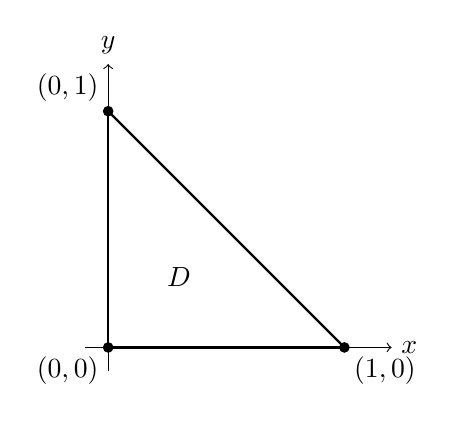
\begin{tikzpicture}[scale=3]
        % Axes
        \draw[->] (-0.1, 0) -- (1.2, 0) node[right] {$x$};
        \draw[->] (0, -0.1) -- (0, 1.2) node[above] {$y$};
        
        % Triangle vertices
        \filldraw[black] (0, 0) circle (0.02) node[below left] {$(0,0)$};
        \filldraw[black] (1, 0) circle (0.02) node[below right] {$(1,0)$};
        \filldraw[black] (0, 1) circle (0.02) node[above left] {$(0,1)$};
        
        % Triangle edges
        \draw[thick] (0, 0) -- (1, 0);
        \draw[thick] (1, 0) -- (0, 1);
        \draw[thick] (0, 1) -- (0, 0);

        % Label for the triangle
        \node at (0.3, 0.3) {$D$};
    \end{tikzpicture}

    Since $f(x, y)$ is certainly nonnegative and integrable in the domain $D$, it remains to show that the integral in the domain $D$ of $f(x, y)$ is 1.

    $$\int\!\!\!\int_D f(x, y) dA = \int_0^1 \int_0^{1 - x} 24xy \cdot dy dx = \int_0^1 12x(1 - x)^2 dx = 1$$

    \part
    Find the marginal probability density functions of $X$ and $Y$. Are $X$ and $Y$ independent?
    \sol
    $$f_X(x) = \int_0^{1 - x} f(x, y) dy = \int_0^{1 - x} 24xy dy = 12x(1 - x)^2 \text{ and by symmetry } f_Y(y) = 12y(1 - y)^2$$

    Notice that
    $$f_X(x)\cdot f_Y(y) = 12^2 xy (1 - x)^2(1 - y)^2 \neq f(x, y) \text{, therefore $X, Y$ are not independent.}$$

    \part
    Find $E(X)$ and Var$(X)$.
    \sol
    $$E(X) = \npint x\cdot f_X(x) dx = \int_0^1 x\cdot 12x(1 - x)^2 dx= \frac{2}{5}$$

    $$E(X^2) = \int_0^1 x^2 \cdot 12x(1 - x)^2 dx = \frac{1}{5}$$

    $$\text{Var}(X) = E(X^2) - E^2(X) = \frac{1}{25}$$
\end{parts}

\newpage
\question
Let $X$ and $Y$ be independent uniformly distributed random variables distributed on the interval $[-1, 1]$. That is,
$$f_{X, Y}(x, y) = \frac{1}{4} \mathbbm{1}_D (x, y) \text{ where } D = [-1, 1] \times[-1, 1]$$

\begin{parts}
    \part
    Find $P(|X| < Y)$.
    \sol
    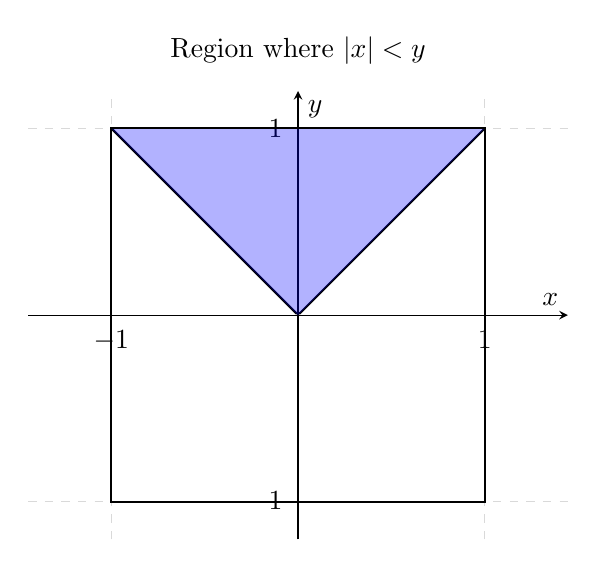
\begin{tikzpicture}
    \begin{axis}[
        axis equal,
        xlabel={$x$},
        ylabel={$y$},
        xmin=-1, xmax=1,
        ymin=-1, ymax=1,
        samples=100,
        title={Region where $|x| < y$},
        axis lines=middle, % Puts the axes at the center
        enlargelimits=true,
        xtick={-1, 0, 1},
        ytick={-1, 0, 1},
        grid=both, % Optional: Add a grid for better visualization
        grid style={dashed, gray!30}
    ]
        % Define y = |x|
        \addplot[domain=-1:1, thick] {abs(x)};
        
        % Shade the region between the upper and lower boundaries
        \fill[blue, opacity=0.3] (-1, 1) -- (1, 1) -- (0, 0);
        
        % Draw the thick outline around the region [-1, 1] x [-1, 1]
        \draw[thick] (-1, -1) rectangle (1, 1);
    \end{axis}
\end{tikzpicture}

$$P(|X| < Y) = \frac{1}{4}\cdot \text{ area of shaded region } = \frac{1}{4}$$


    \part
    Find $P(X^2 < Y^2)$.
    \sol
    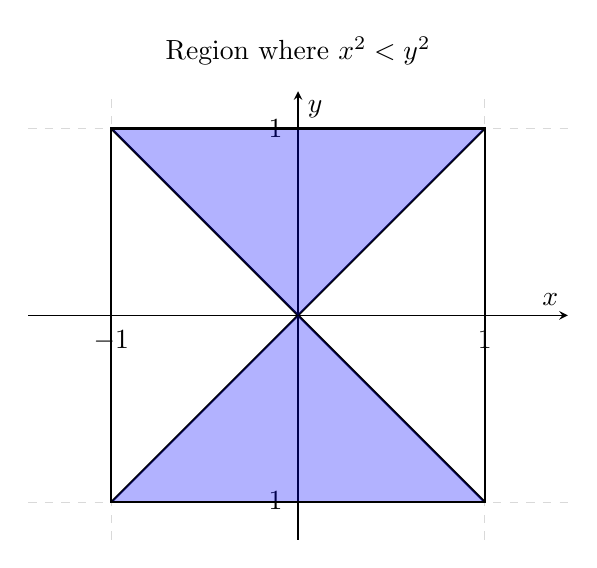
\begin{tikzpicture}
    \begin{axis}[
        axis equal,
        xlabel={$x$},
        ylabel={$y$},
        xmin=-1, xmax=1,
        ymin=-1, ymax=1,
        samples=100,
        title={Region where $x^2 < y^2$},
        axis lines=middle, % Puts the axes at the center
        enlargelimits=true,
        xtick={-1, 0, 1},
        ytick={-1, 0, 1},
        grid=both, % Optional: Add a grid for better visualization
        grid style={dashed, gray!30}
    ]
        % Define y = x
        \addplot[domain=-1:1, thick] {x};
        \addplot[domain=-1:1, thick] {-x};
        
        % Shade the region between the upper and lower boundaries
        \fill[blue, opacity=0.3] (-1, -1) -- (0, 0) -- (1, -1);
        \fill[blue, opacity=0.3] (-1, 1) -- (0, 0) -- (1, 1);
        
        % Draw the thick outline around the region [-1, 1] x [-1, 1]
        \draw[thick] (-1, -1) rectangle (1, 1);
    \end{axis}
\end{tikzpicture}

$$P(X^2 < Y^2) = \frac{1}{4} \cdot \text{ area of shaded region } = \frac{1}{2}$$


\end{parts}



\newpage
\question
Let $X, Y$ be independent random variables uniformly distributed on the interval $[-1, 1]$. That is,

$$f_X(x) = f_Y(x) = \frac{1}{2} \mathbbm{1}_{[-1, 1]}(x)$$

Let $Z = X + Y$

\begin{parts}
    \part
    Find the probability density function of $Z$.
    \sol
    $$f_Z(z) = \npint f_X(x)f_Y(z - x)dx = \npint \frac{1}{4} \cdot \mathbbm{1}_{[-1, 1]}(x) \mathbbm{1}_{[-1, 1]}(z - x)$$

    Examing the indicator functions tells us that
    $$-1 \leq x \leq 1, \text{ and }$$
    $$-1 \leq z - x \leq 1 \longrightarrow z - 1 \leq x \leq z + 1$$

    We can then rewrite out bounds of the integral as the minimum$(-1, z - 1)$ and the maximum$(1, z + 1)$.

    $$f_Z(z) = \int_{\min (-1, z - 1)}^{\max (1, z + 1)} \frac{1}{4}dx =
    \begin{cases}
        \frac{1}{4}\int_{-1}^{z + 1}dx = \frac{2 + z}{4}, & z \leq 0 \\
        \frac{1}{4}\int_{z - 1}^{1}dx = \frac{2 - z}{4}, & z \geq 0 \\
    \end{cases}$$

    \part
    Check that $\npint f_Z(z) dz = 1$.
    \sol
    $$\npint f_Z(z)dz = \int_{-2}^2 f_Z(z)dz = \int_{-2}^0 \frac{2 + z}{4}dz + \int_0^2 \frac{2 - z}{4}dz = \frac{1}{2} + \frac{1}{2} = 1$$

    \part
    Find $E(Z)$ and Var$(Z)$.
    \sol
    $$E(Z) = \int_{-2}^2 zf_Z(z)dz = \int_{-2}^0 z\cdot \frac{2 + z}{4}dz + \int_0^2 z\cdot \frac{2 - z}{4}dz = -\frac{1}{3} + \frac{1}{3} = 0$$

    $$E\paren{Z^2} = \int_{-2}^2 z^2\cdot f_Z(z)dz = \int_{-2}^0 z^2\cdot \frac{2 + z}{4}dz + \int_0^2 z^2\cdot \frac{2 - z}{4}dz = \frac{1}{3} + \frac{1}{3} = \frac{2}{3}$$

    $$\text{Var}(Z) = E\paren{Z^2} - E^2(Z) = \frac{2}{3}$$
\end{parts}



\newpage
\question
Let $U \sim$ Uniform$[0, 1]$ and $T \sim$ Exp$(1)$ with $U,T$ independent. Define $Z = U + T$.

\begin{parts}
    \part
    Find the probability density function of $Z$.
    \sol
    $$f_Z(z) = \npint f_T(x)f_U(z - x)dx = \npint e^{-x} \cdot \mathbbm{1}_{[0, \infty)}(x) \mathbbm{1}_{[0, 1]}(z - x) dx$$

    Examining the indicator functions tells us that
    $$0 \leq x < \infty \text{ and }$$
    $$0 \leq z - x \leq 1 \longrightarrow z - 1 < x < z$$

    We rewrite the bounds of the integral as maximum$(0, z - 1)$ and minimum$(\infty, z) = z$.

    $$f_Z(z) = \int_0^{\max (1, z)} e^{-x} dx =
    \begin{cases}
        \int_0^z e^{-x} dx = -e^{-z} + 1, & z \leq 1 \\
        \int_{z - 1}^z e^{-x} dx = -e^{-z} + e^{-(z - 1)}, & z \geq 1 \\
    \end{cases}$$


    \part
    Check that $\npint f_Z(z)dz = 1$.
    \sol
    $$\npint f_Z(z) dz = \int_0^1 -e^{-z} + 1 dz + \int_1^\infty -e^{-z} + e^{-(z - 1)} dz = \paren{e^{-1} - 1 + 1} + \paren{-e^{-1} + 1} = 1$$



    \part
    Find $E(Z)$ and $\text{Var}(Z)$.
    \sol
    $$E(Z) = \int_0^1 z\cdot \paren{-e^{-z} + 1} dz + \int_1^\infty z\cdot \paren{-e^{-z} + e^{-(z - 1)}} dz = \paren{2e^{-1} - \frac{1}{2}} + \paren{-2e^{-1} + 2} = \frac{3}{2}$$

    $$E\paren{Z^2} = \int_0^1 z^2\cdot (-e^{-z} + 1)dz + \int_1^\infty z^2\cdot (-e^{-z} + e^{-(z - 1)}) dz = \paren{5e^{-1} - \frac{5}{3}} + \paren{-5e^{-1} + 5} = \frac{10}{3}$$

    $$\text{Var}(Z) = E\paren{Z^2} - E^2(Z) = \frac{10}{3} - \paren{\frac{3}{2}}^2 = \frac{13}{12}$$
\end{parts}


\newpage
\question
Particles are subject to collisions which cause them to split into two parts, each part taking a fraction of the parent mass. Suppose that this fraction is uniformly distributed on the interval $[0, 1]$. Following a single particle through several splittings, we obtain a fraction of the original particle
$$Z_n = X_1 \cdot \hdots \cdot X_n \text{ where }\cbrac{X_j}_{j = 1}^\infty \text{ are iid uniformly distributed on }[0, 1] \text{ random variables}$$

\begin{parts}
    \part
        Show that the density for a random variable $T_1 = -\ln (X_1)$ is an exponential random variable with parameter $\lambda = 1$.
        \begin{proof}
        Since $T_1 = -\ln (X_1)$, we can rearrange the variables into
        $$X_1 = e^{-T_1}, \frac{dX_1}{dT_1} = -e^{-T_1}$$
    
        We can find the pdf of $T_1$ by writing it in terms of $X_1$ and correcting it with the Jacobian.
        $$f_{T_1}(t) = f_{X_1}(x)\cdot \abs{\frac{dX_1}{dT_1}} = \mathbbm{1}_{[0, 1]}(x)\cdot \abs{-e^{-t}} = e^{-t}\mathbbm{1}_{[0, \infty)}(t)$$
    \end{proof}

    


    \part
    We know that the sum of independent exponential random variables with parameter $\lambda$ has a Gamma distribution. That is, for $n \geq 1$, set
    $$Y_n = \sum_{j = 1}^n T_j \text{ where } \cbrac{T_j}_{j = 1}^\infty \text{ are iid } T_1 \sim \text{Exp}(\lambda), \text{ then}$$

    $$f_{Y_n}(t) = \frac{(\lambda t)^{n - 1}}{(n - 1)!} \lambda e^{-\lambda t} \mathbbm{1}_{[0, \infty)}(t)$$

    Show that
    $$f_{Z_n}(z) = \frac{1}{(n - 1)!}(-\ln (z))^{n - 1} \mathbbm{1}_{[0, 1]}(z)$$
    \begin{proof}
        Before any proof, note that some simple computations will yield
        $$Y_n = T_1 + \hdots + T_n = -\ln X_1 - \hdots -\ln X_n = \ln X_1^{-1} + \hdots + \ln X_n^{-1} = \ln (X_1 \cdots \hdots \cdots X_n)^{-1} =$$
        $$= \ln \frac{1}{Z_n} = -\ln Z_n, \longrightarrow Y_n = -\ln Z_n, \abs{\frac{dY_n}{dZ_n}} = \frac{1}{Z_n}, \text{ and }t = -\ln z$$


        Again, to derive a pdf for $Z_n$, we will use the pdf of $Y_n$ and use the Jacobian to correct.
        $$f_{Z_n}(z) = f_{Y_n}(t) \cdot \abs{\frac{dY_n}{dZ_n}} = \frac{t^{n - 1}}{(n - 1)!}e^{-t}\cdot \frac{1}{z}\mathbbm{1}_{[0, \infty)}(t), \text{ and plugging in } t = -\ln z \text{ gives}$$

        $$f_{Z_n}(z) = \frac{(-\ln z)^{n - 1}}{(n - 1)!}\cdot e^{\ln z}\cdot \frac{1}{z} \mathbbm{1}_{[0, 1]}(z)= \frac{(-\ln z)^{n - 1}}{(n - 1)!}\mathbbm{1}_{[0, 1]}(z)$$
    \end{proof}
\end{parts}
\end{questions}

\end{document}